\RequirePackage{luatex85}
\documentclass{standalone}
\usepackage{amssymb,amsmath}
\usepackage{tikz}
\usetikzlibrary{automata,positioning}
\begin{document}
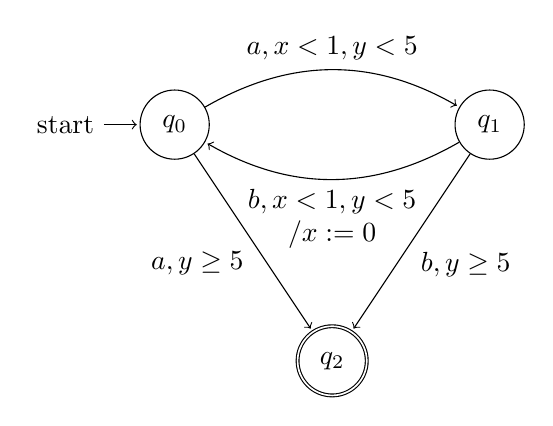
\begin{tikzpicture}[shorten >=1pt,node distance=4cm,on grid,auto] 
 \node[state,initial] (q_0) {$q_0$};
 \node[state] (q_1)[right=of q_0] {$q_1$};
 \node[state,accepting] (q_2) at (2,-3) {$q_2$};
 \path[->]
 (q_0) edge[bend left] node{$a,x<1,y<5$} (q_1)
 (q_1) edge[bend left] node[align=center] {$b,x<1,y<5$\\ $/x:=0$} (q_0)
 (q_0) edge [below left] node[align=center] {$a,y\geq5$} (q_2)
 (q_1) edge [below right] node[align=center] {$b,y\geq5$} (q_2);
\end{tikzpicture} 
 \end{document}